\documentclass[conference]{IEEEtran}
%\IEEEoverridecommandlockouts
% The preceding line is only needed to identify funding in the first footnote. If that is unneeded, please comment it out.
%Template version as of 6/27/2024

\usepackage{cite}
\usepackage{amsmath,amssymb,amsfonts}
\usepackage{algorithmic}
\usepackage{graphicx}
\usepackage{textcomp}
\usepackage{xcolor}
\def\BibTeX{{\rm B\kern-.05em{\sc i\kern-.025em b}\kern-.08em
    T\kern-.1667em\lower.7ex\hbox{E}\kern-.125emX}}
\begin{document}

\title{A Dual-Tier Edge-Cloud Architecture for Real-Time Basketball Activity Recognition and Fatigue Monitoring.\\
%{\footnotesize \textsuperscript{*}Note: Sub-titles are not captured for https://ieeexplore.ieee.org  and should not be used}
%\thanks{Identify applicable funding agency here. If none, delete this.}
}

\author{\IEEEauthorblockN{1\textsuperscript{st} Ricardo Monteiro}
\IEEEauthorblockA{\textit{Dept. of Electrical Engineering} \\
\textit{Faculty of Sciences and Technology (FCT)}\\
Universidade Nova de Lisboa, Caparica, Portugal}% \\
%email address or ORCID}
\and
\IEEEauthorblockN{2\textsuperscript{nd} Anikó Costa}
\IEEEauthorblockA{\textit{Dept. of Electrical Engineering} \\
\textit{Faculty of Sciences and Technology (FCT)}\\
Universidade Nova de Lisboa, Caparica, Portugal}% \\
%email address or ORCID}
%\and
%\IEEEauthorblockN{3\textsuperscript{rd} Given Name Surname}
%\IEEEauthorblockA{\textit{dept. name of organization (of Aff.)} \\
%\textit{name of organization (of Aff.)}\\
%City, Country \\
%email address or ORCID}
%\and
%\IEEEauthorblockN{4\textsuperscript{th} Given Name Surname}
%\IEEEauthorblockA{\textit{dept. name of organization (of Aff.)} \\
%\textit{name of organization (of Aff.)}\\
%City, Country \\
%email address or ORCID}
%\and
%\IEEEauthorblockN{5\textsuperscript{th} Given Name Surname}
%\IEEEauthorblockA{\textit{dept. name of organization (of Aff.)} \\
%\textit{name of organization (of Aff.)}\\
%City, Country \\
%email address or ORCID}
%\and
%\IEEEauthorblockN{6\textsuperscript{th} Given Name Surname}
%\IEEEauthorblockA{\textit{dept. name of organization (of Aff.)} \\
%\textit{name of organization (of Aff.)}\\
%City, Country \\
%email address or ORCID}
}

\maketitle

\begin{abstract}
Traditional sports wearables rely predominantly on kinematic data from Inertial Measurement Units (IMUs), lacking the physiological context required to classify complex movements and detect muscle fatigue. This 
paper presents a multi-modal wearable ecosystem designed for basketball analytics, fusing 9-axis IMU data with Electromyography (EMG) via a bilateral footwear prototype. The system utilizes a 
dual-tier architecture: a quantized TinyML neural network executing locally on an Android edge-computing hub for real-time inference, and a cloud-based Random Forest classifier for deep post-session analysis. 
Empirical evaluation demonstrates that EMG features, specifically Variance and RMS, are the primary predictors for movement classification, outperforming traditional kinematics. During live testing, the localized 
TinyML model achieved 79.5\% accuracy, outperforming the cloud-tier model while eliminating network latency. Furthermore, a 500ms majority-voting smoothing algorithm increased classification stability by 6.4\%, 
providing a robust framework for real-time athletic monitoring and fatigue-based injury prevention.
\end{abstract}

\begin{IEEEkeywords}
Wearables, Sensor Fusion, EMG, IMU, Edge ML, TinyML, Basketball Analytics.
\end{IEEEkeywords}

\section{Introduction}

The constant pursuit of efficiency and durability extends not only to technology but also to human performance. Central to this 
evolution is the rapid progression of wearable technology, which has transitioned from simple step-counting peripherals to sophisticated diagnostic tools. These devices now 
encompass a vast range of applications, including medical diagnostics, injury prevention, sleep analysis, and high-fidelity sports performance monitoring.

In recent years, the synergy between advanced microcontrollers and smartphone has revolutionized the sports landscape. Modern athletics is increasingly defined by 
data-driven decision-making, where statistics are utilized to gain competitive advantages. However, as the demand for deeper insights grows, the complexity of the 
data required to satisfy these metrics has increased proportionally.

Compared to single-activity recognition, team sports present significant challenges for real-time analytics. The inherent unpredictability, 
high-intensity intervals, and constant physical interaction between players create a volatile data environment. These sports are characterized by explosive, short-duration 
movements and high levels of physiological stress, especially during a game's climax where the risk of injury is most prevalent~\cite{b1}.

Despite these advancements, standard sports wearables remain limited by their reliance on single-modality sensing, typically utilizing only Inertial Measurement Units (IMU). 
While kinematics provide a trajectory of movement, they lack the neuromuscular context required to differentiate between explosive intent and mere mechanical motion. 
Furthermore, the reliance on cloud-based processing introduces latency that can be critical in injury-prevention scenarios.

This paper addresses these gaps by proposing a multi-modal, dual-tier architecture that fuses IMU kinematics with Electromyography (EMG). By leveraging Edge AI for 
localized inference on a mobile hub, the system provides a low-latency solution for movement classification and fatigue monitoring, ensuring that the physiological cost of 
movement is captured as accurately as its physical path.


\section{Related Work}
\label{related_work}

The development of intelligent sports wearables has increasingly focused on objective physiological monitoring to supplement traditional kinematic tracking. Recent research 
demonstrates a paradigm shift toward multi-modal sensor fusion and edge-based analytics to enhance the accuracy of activity recognition and fatigue detection.

A common challenge in athletic monitoring is the inability of single-modality sensors to provide full biomechanical context. Hwang et al. addressed this by integrating surface 
electromyography (sEMG) and inertial measurement units (IMU) to classify physical fatigue during natural over-ground walking. Their hybrid CNN-LSTM-Attention model, evaluated 
via leave-one-subject-out cross-validation, achieved 87.94\% accuracy, proving that combining physiological markers from the gastrocnemius with kinematic jerk signals significantly 
enhances system robustness against individual variability~\cite{b6}. Similarly, Otálora et al. demonstrated that for upper limb fatigue estimation during repetitive lifting, a combination 
of IMUs and Optical Fiber Sensors (OFS) achieved 95.4\% accuracy. Their findings highlight that while EMG is a gold standard for bio-electrical muscle function, its reliability 
in long-term work environments can be compromised by factors like skin perspiration, making supplemental kinematic data essential~\cite{b9}.

The choice of classifier and processing pipeline is critical for real-time mobile deployment. Baigarayeva et al. developed an IoT-based system, "Qimyl," which performs on-device 
feature extraction (RMS, MAV, MDF) to classify muscle fatigue during sustained isometric tasks. By comparing logistic regression, decision trees (DT), and XGBoost, they identified 
DT as achieving the highest accuracy (90.7\%) for their specific submaximal grip tasks. Furthermore, their work emphasizes the value of synchronizing objective EMG features 
with subjective self-assessments (e.g., the Borg scale) to improve the ecological validity of the models~\cite{b5}.

Beyond standard classification, researchers have explored deterministic indices to objectively detect the moment of failure. Qassim et al. proposed a double-step binary 
classifier utilizing a new fatigue index based on the difference between high-frequency and low-frequency components of the sEMG signal. This algorithm achieved 94.66\% 
accuracy in identifying the moment a muscle fails to sustain required force, providing a blueprint for active injury-prevention alerts~\cite{b2}. These findings are supported by 
Kamaruddin et al., whose review of surface electromyography emphasizes that while time-domain features like Waveform Length (WL) offer low computational complexity, 
frequency-domain analysis remains superior for quantifying the physiological shift to lower frequencies that characterizes neuromuscular fatigue~\cite{b4}.


\section{System Architecture}
\label{system_architecture}

The proposed system follows a decentralized, multi-modal architecture designed to bridge localized physiological sensing with high-level cloud analytics. The framework is 
divided into three primary layers: the sensor-embedded hardware, the mobile edge-computing hub, and the cloud-based inference server (Fig.~\ref{system_architecture}).

\begin{figure*}[htbp]
\centerline{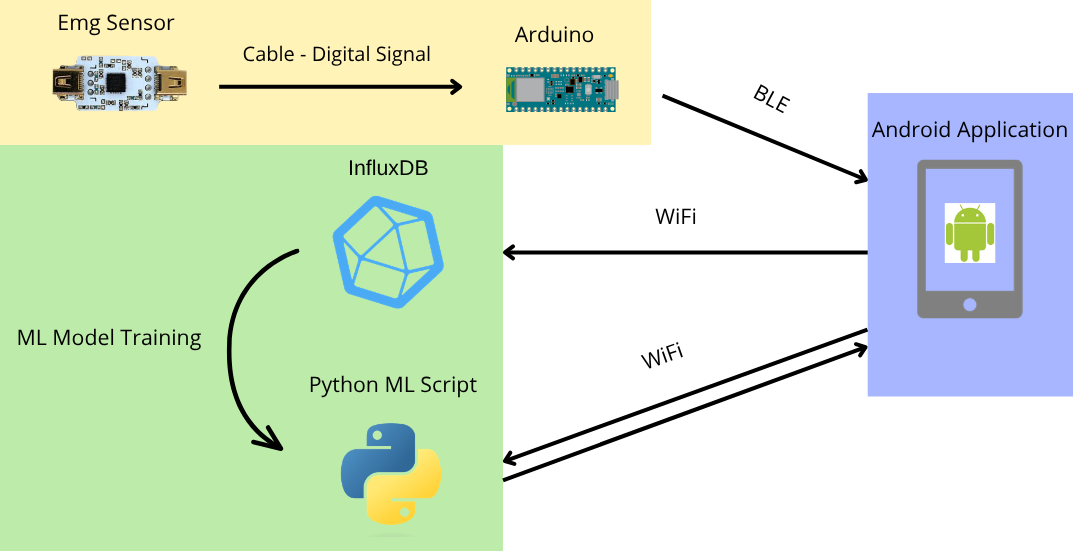
\includegraphics[width=0.9\textwidth]{System_Overview.jpg}}
\caption{System Overview.}
\label{systemOverview}
\end{figure*}

\subsection{Hardware Prototype}

The sensory layer consists of two footwear-mounted prototypes. Each unit is centered around an Arduino Nano 33 BLE Sense Rev2, chosen for its embedded 9-axis Inertial 
Measurement Unit (IMU) and Bluetooth Low Energy (BLE) module (Fig.~\ref{prototype}). To provide physiological context, a localized Electromyography (EMG) sensor is integrated into each module to monitor 
the electrical activity of the Gastrocnemius Lateralis.


The firmware implements a non-blocking sampling strategy. To maintain sampling periodicity despite the periodic blocking of the BLE radio stack, a microsecond-precision hardware timer tracks "time debt." If a 
transmission delays the loop, a sequential catch-up routine is executed to preserve the 1ms EMG sampling interval.

To overcome the bandwidth limitations associated with transmitting raw high-frequency raw EMG data, six EMG features are sent instead. Every 20 ms, the system samples the IMU data and computes the six
time-domain features using a 200ms sample window (N=200):

Root Mean Square (RMS): Represents the signal power and is defined as:
\begin{equation} 
  RMS = \sqrt{\frac{1}{N} \sum_{i=1}^{N} x_i^2} 
\end{equation}

Variance (VAR): Measures the power of the AC component of the EMG signal:
\begin{equation}
  VAR = \frac{1}{N - 1} \sum_{i = 1}^{N} (x_i - \mu)^2
\end{equation}

Mean Absolute Value (MAV): An indicator of muscle contraction levels.
\begin{equation}
  MAV = \frac{1}{N} \sum_{i = 1}^{N} \left\lvert x_i \right\rvert 
\end{equation}

Waveform Length (WL): Captures the cumulative complexity of the signal's amplitude, frequency, and duration.

\begin{equation}
  WL = \sum_{i = 1}^{N - 1} \lvert x_{i + 1} - x_i \rvert
\end{equation}

Zero Crossing (ZC) and Slope Sign Change (SSC): These provide a simple representation of the frequency domain properties in the time domain, helping to identify shifts in muscle firing rates.

\begin{equation}
  ZC = \begin{cases}
    \sum_{n = 2}^{N} sgn(x_i \cdot x_{i-1})
    (x_i - x_{i-1}) \geq \epsilon 
  \end{cases}
\end{equation}

\begin{equation}
  sgn(x) = \begin{cases}
    1 & \text{if }  x > \epsilon \\
    0 & \text{otherwise}
  \end{cases}
\end{equation}

\begin{equation}
  SSC = \sum_{i = 2}^{N - 1} f[(x_i - x_{i-1}) \cdot (x_i - x_{i+1})]
\end{equation}

To optimize BLE bandwidth, the system bundles five 30-byte frames into a single 150-byte payload, transmitted to the mobile hub every 100 ms.


\begin{figure}[b]
\centerline{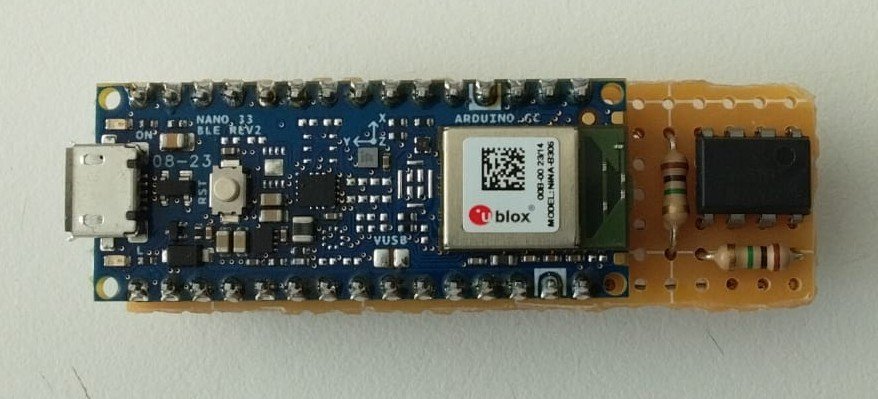
\includegraphics[width=0.9\linewidth]{deviceTop.jpg}}
\caption{Prototype Picture.}
\label{prototype}
\end{figure}

\subsection{Android Application and Data Synchronization}

The center of the proposed architecture is a native Android application developed in Kotlin using the Model-View-ViewModel (MVVM) architecture. It serves as the bridge between the user and the prototypes, handling 
the bilateral data synchronization. When the app receives the BLE communications from the left or right device, it separates the five received data bundles and assigns time-stamps to each proceeding to forward them 
to the cloud InfluxDB data base.

Beyond data processing, the application manages individualized user profiles that may ensure personalized monitoring in future iterations and the sensors' calibration. To maintain high performance during intense 
activity, the application utilizes asynchronous background threads for inference and cloud synchronization, ensuring the real-time activity dashboard remains responsive.

\subsection{Temporal Smoothing and Output Stability}

To handle the inherent mechanical noise of high-intensity basketball movements, the system utilizes a 300 ms sliding window with a 100 ms step size for feature aggregation. A critical contribution of this 
architecture is the implementation of a post-processing temporal smoothing layer. Utilizing a continuous sliding window (implemented via an \textit{ArrayDeque}), a Majority Voting algorithm evaluates the last five 
local predictions, providing a 500 ms context. This logic acts as a digital low-pass filter, effectively eliminating prediction "flickering" and hardware-induced false positives, thereby ensuring a stable and 
reliable stream of activity classifications during steady-state movements.


\subsection{Dual-Tier Machine Learning}

The architecture employs a dual-tier approach, for movement recognition, to compare latency and model complexity:

\begin{itemize}
  \item Edge Tier (TinyML): A lightweight, quantized Neural Network (NN) is embedded directly within the Android application using TensorFlow Lite. This model provides ultra-low latency inference, enabling real-time feedback and driving the deterministic injury-prevention algorithm independently of network availability.
  \item Cloud Tier (Random Forest): Simultaneously, the 300 ms window is serialized into a JSON payload and transmitted via an asynchronous HTTP POST request to a Flask-based server. The server hosts a high-dimensional Random Forest (RF) classifier used for deep analysis and comparative validation against the edge model.
\end{itemize}


\subsection{Fatigue Monitoring and Warning}

Beyond activity classification, the system implements a real-time monitoring layer designed to identify early indicators of neuromuscular fatigue. This functionality is supported by the observation that localized 
muscle fatigue manifests as a measurable increase in the amplitude of the EMG signal, due to the need of higher muscle effort to maintain force output.

The monitoring logic operates on a threshold-based trigger system integrated within the Android app. This threshold is personal and a calibration should be performed in the beginning of every session. For this paper, 
only one player was tested so only one threshold was calculated and the calibration wasn't implemented. The threshold value was calculated by monitoring the athlete at the beginning of practice (with relaxed muscles) 
and when he was almost cramping and comparing the data while idling or walking.

To prevent false positives caused by mechanical spikes or explosive movements (such as a single rebound), the alert logic requires a temporal persistence of high-intensity sEMG activity. A warning is only 
triggered if the physiological features exceed the pre-set threshold for a continuous duration of 1 second. Once these conditions are met, the application provides immediate feedback with a visual alert on the 
dashboard, enabling the athlete or coach to make informed decisions regarding rest and injury prevention.


\section{Experimental Method and Results}
\label{results}

\subsection{Experimental Method}
The system was evaluated through a series of dynamic basketball drills involving several volunteer subjects. The dataset was partitioned into an 80/20 train-test split to 
validate the classification models across five macro-movements: Idle, Walking, Running, Defensive Slide, and Rebound. The cramping prevention system
was only tested on one player that pushed his muscles to near involuntary contractions.

The prototypes were mounted directly in the athletes' footwear to approximate the ideal
positioning(on the bottom of the feet as an insole or a sock). The devices were secured using
the shoe laces and the powerbank was secured in the users socks, utilizing the existing
infrastructure. With this configuration, the IMU accurately captures the kinematics of
the foot, such as accelerations and rotational velocities during the athletes' movements.
Furthermore, this setup minimizes the mechanical strain exerted by the power cables on
the USB ports, while keeping the EMG leads in close proximity to the chosen muscle
group. 

The muscle chosen to be measured was the Gastrocnemius Lateralis as it is one of the most important muscles for explosive jumping motion. The position for the EMG
sensors was chosen as recommended by the European Union (EU)'s SENIAM (Surface ElectroMyoGraphy for the Non-Invasive Assessment of Muscles) project (~\cite{b7}) ensuring standardization and maximization of the 
signal-to-noise ratio.

To ensure correct labeling for the supervised learning models, a manual annotation interface was integrated into the mobile application. Data collection was performed in controlled sessions where the 
athlete executed specific basketball movements while researcher chose the correct label and turned a "Send data" switch within the Android UI.

When the switch was activated, the application bundled the incoming 30-feature sensor vector with the corresponding label (e.g., Defensive Sliding or Running), user ID and time, before transmitting the packet to the 
InfluxDB database.

\subsection{Model Training and Convergence}

The TinyML model demonstrated robust learning, achieving a validation accuracy of approximately 94% with synchronized descent in categorical cross-entropy loss, indicating 
high generalization. Conversely, the Cloud-based Random Forest (RF) was evaluated using ROC and Precision-Recall curves. The Area Under the Curve (AUC) for all classes 
approached 1.0, and the PR curves confirmed the model's ability to handle the class imbalance inherent in basketball data (e.g., rare rebounding events vs. frequent 
running/walking).

\subsection{Feature Importance and Sensor Contribution}

A core contribution of this work is the validation of EMG integration. Gini Feature Importance analysis (Fig.~\ref{featureImportance}) revealed that EMG-derived features, specifically Variance 
(VAR) and Root Mean Square (RMS), were the primary contributors to classification accuracy. This confirms that physiological electrical activity provides critical intent-based 
context that kinematics alone lack. Additionally, the model exhibited a preference for features from the dominant (left) limb, successfully capturing subject-specific 
biomechanical asymmetries.

\begin{figure}[b]
\centerline{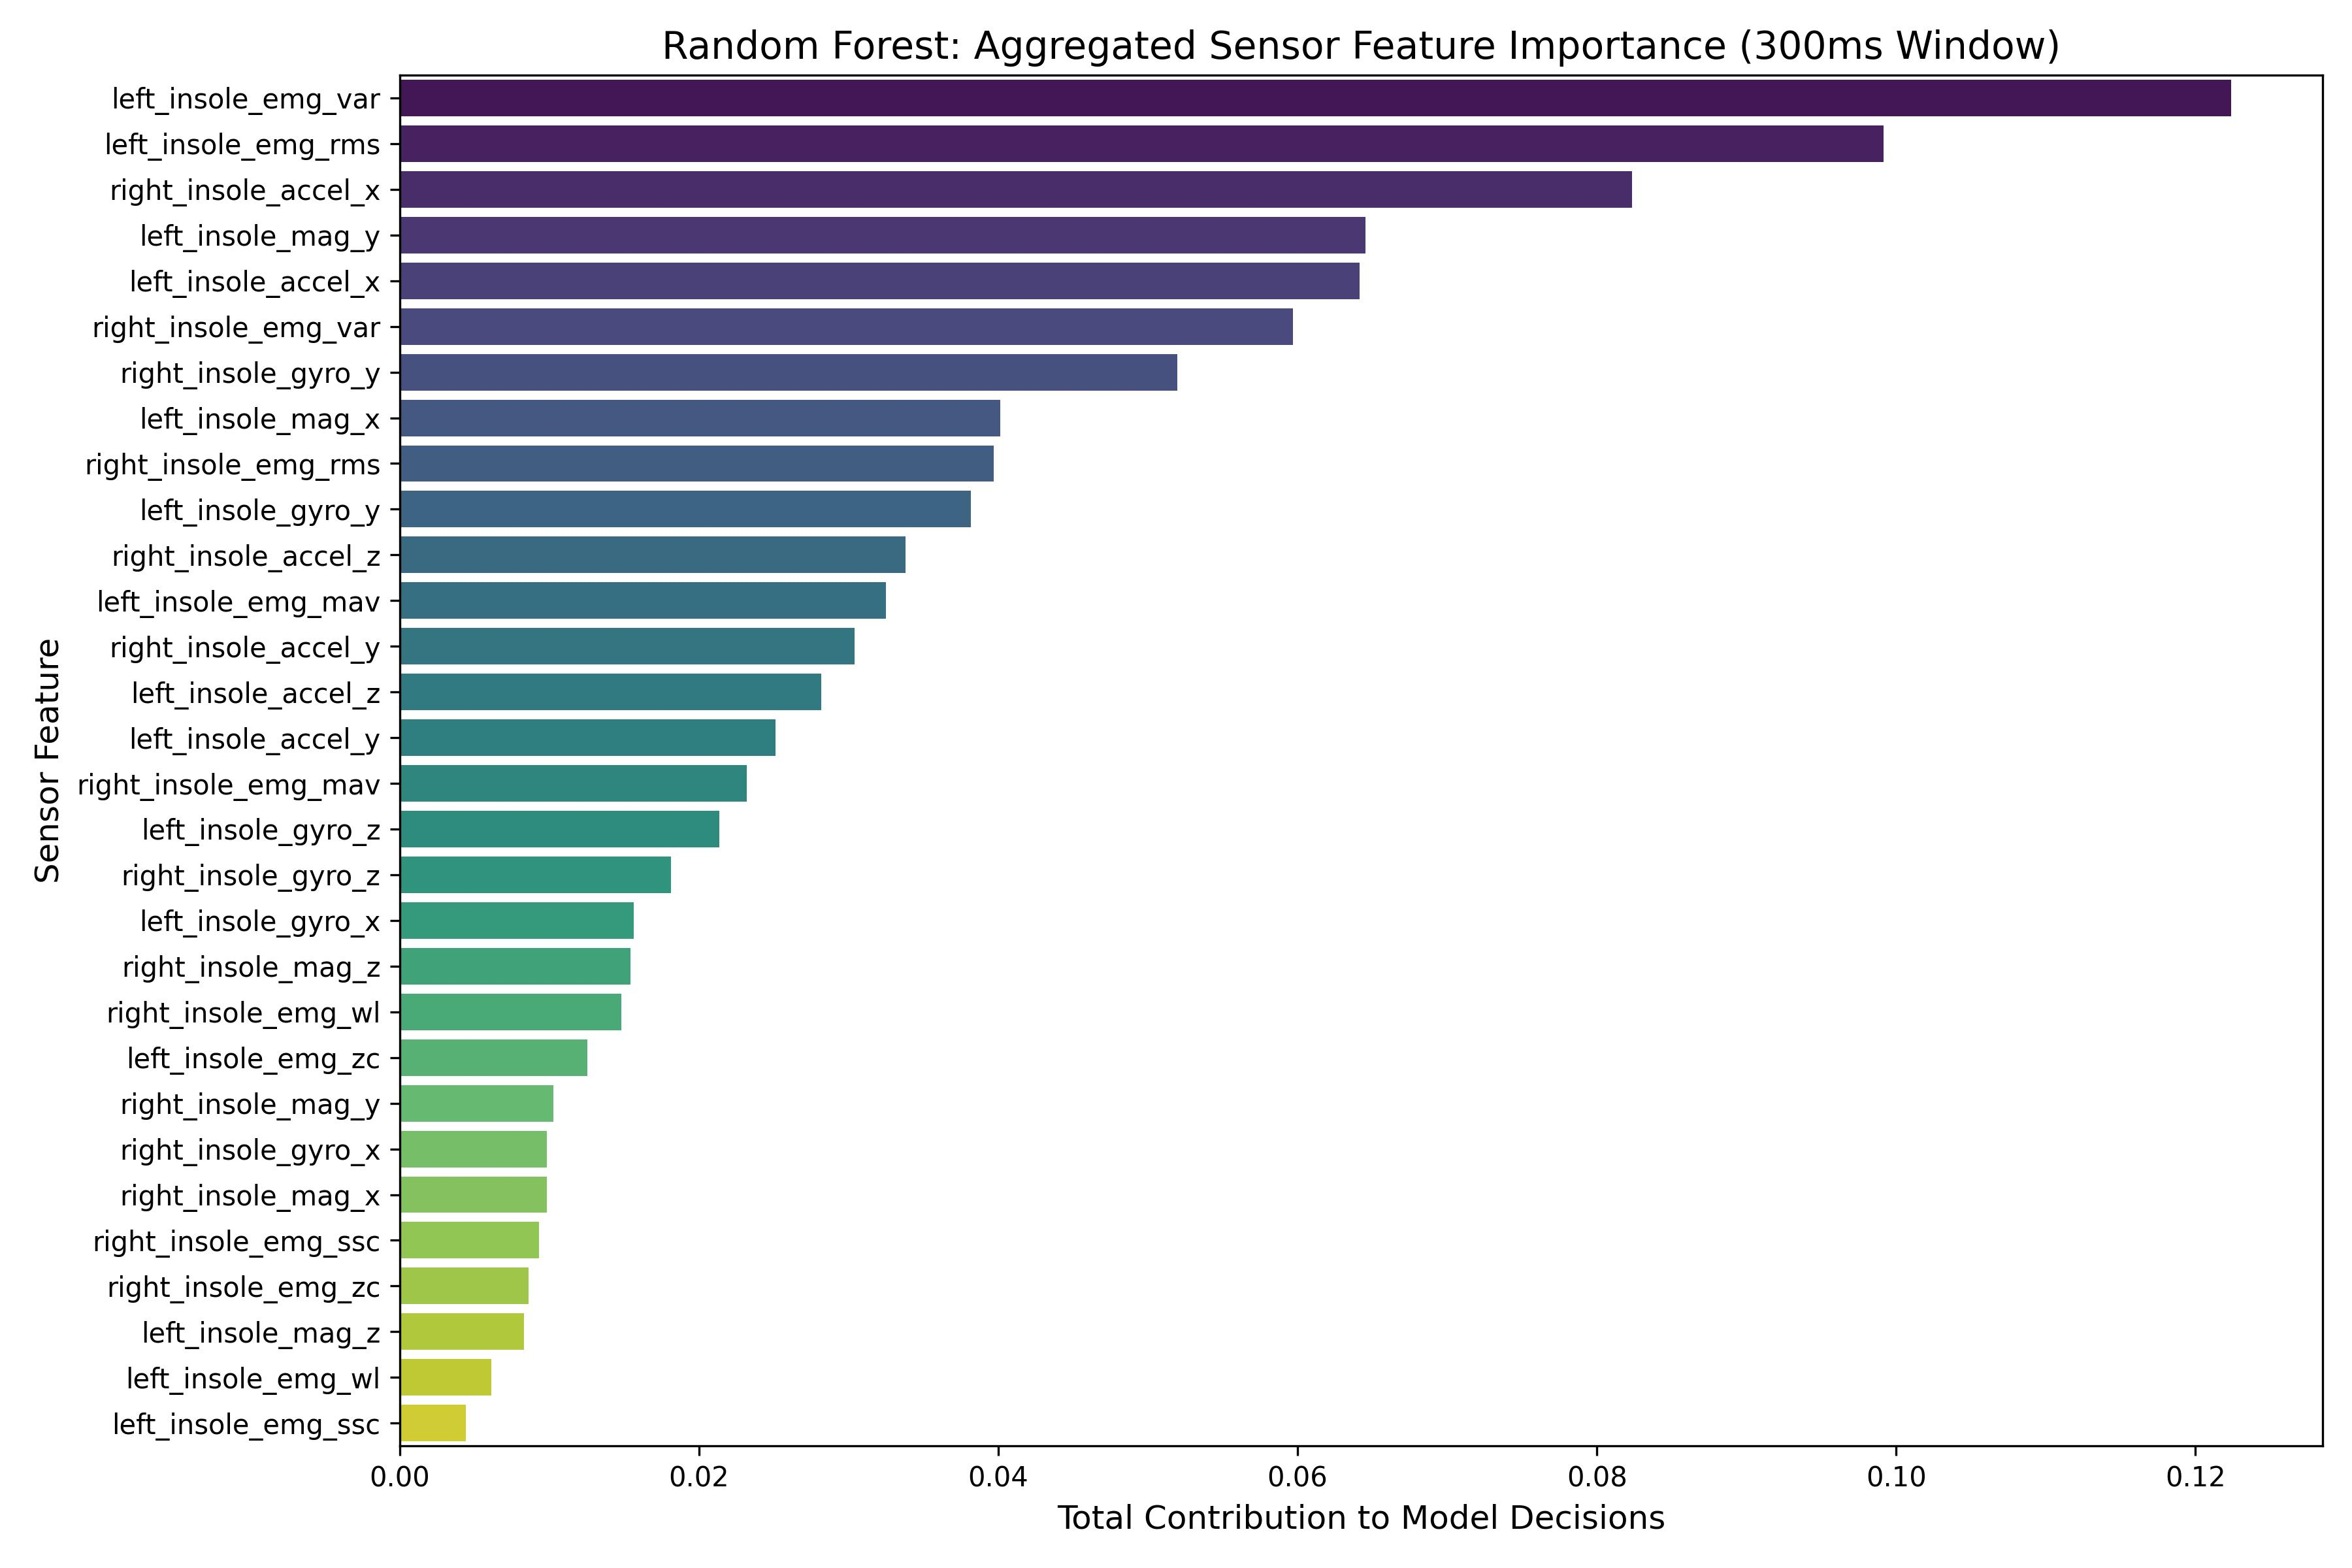
\includegraphics[width=\linewidth]{featureImportance.jpg}}
\caption{Feature Importance.}
\label{featureImportance}
\end{figure}

\subsection{Edge vs. Cloud: Real-Time Performance}

During live testing, the localized TinyML model outperformed the Cloud RF model, achieving an overall accuracy of 79.5\% compared to the server's 71.2\%. While the RF model 
excelled at slower movements (Idle, Walking), it struggled with dynamic transitions in the field. Notably, the TinyML model provided instantaneous inference, whereas 
the RF model introduced measurable network latency.

\subsection{Temporal Smoothing Improvements}

The 500ms majority-voting algorithm provided a significant stability boost. For the TinyML model, smoothing increased overall accuracy by 6.4\% by acting as a digital low-pass 
filter that neutralized prediction flickering. Confusion matrix analysis (Fig.~\ref{CFRaw}, Fig.~\ref{CFSmoothed}) shows that while smoothing improved steady-state detection, it reduced sensitivity to 
transient events like "Rebounding," which were often outvoted by surrounding states. This identifies a fundamental trade-off: smoothing is essential for consistent 
activity tracking but may require dynamic windowing for explosive event detection in future iterations.

\begin{figure}[b]
\centerline{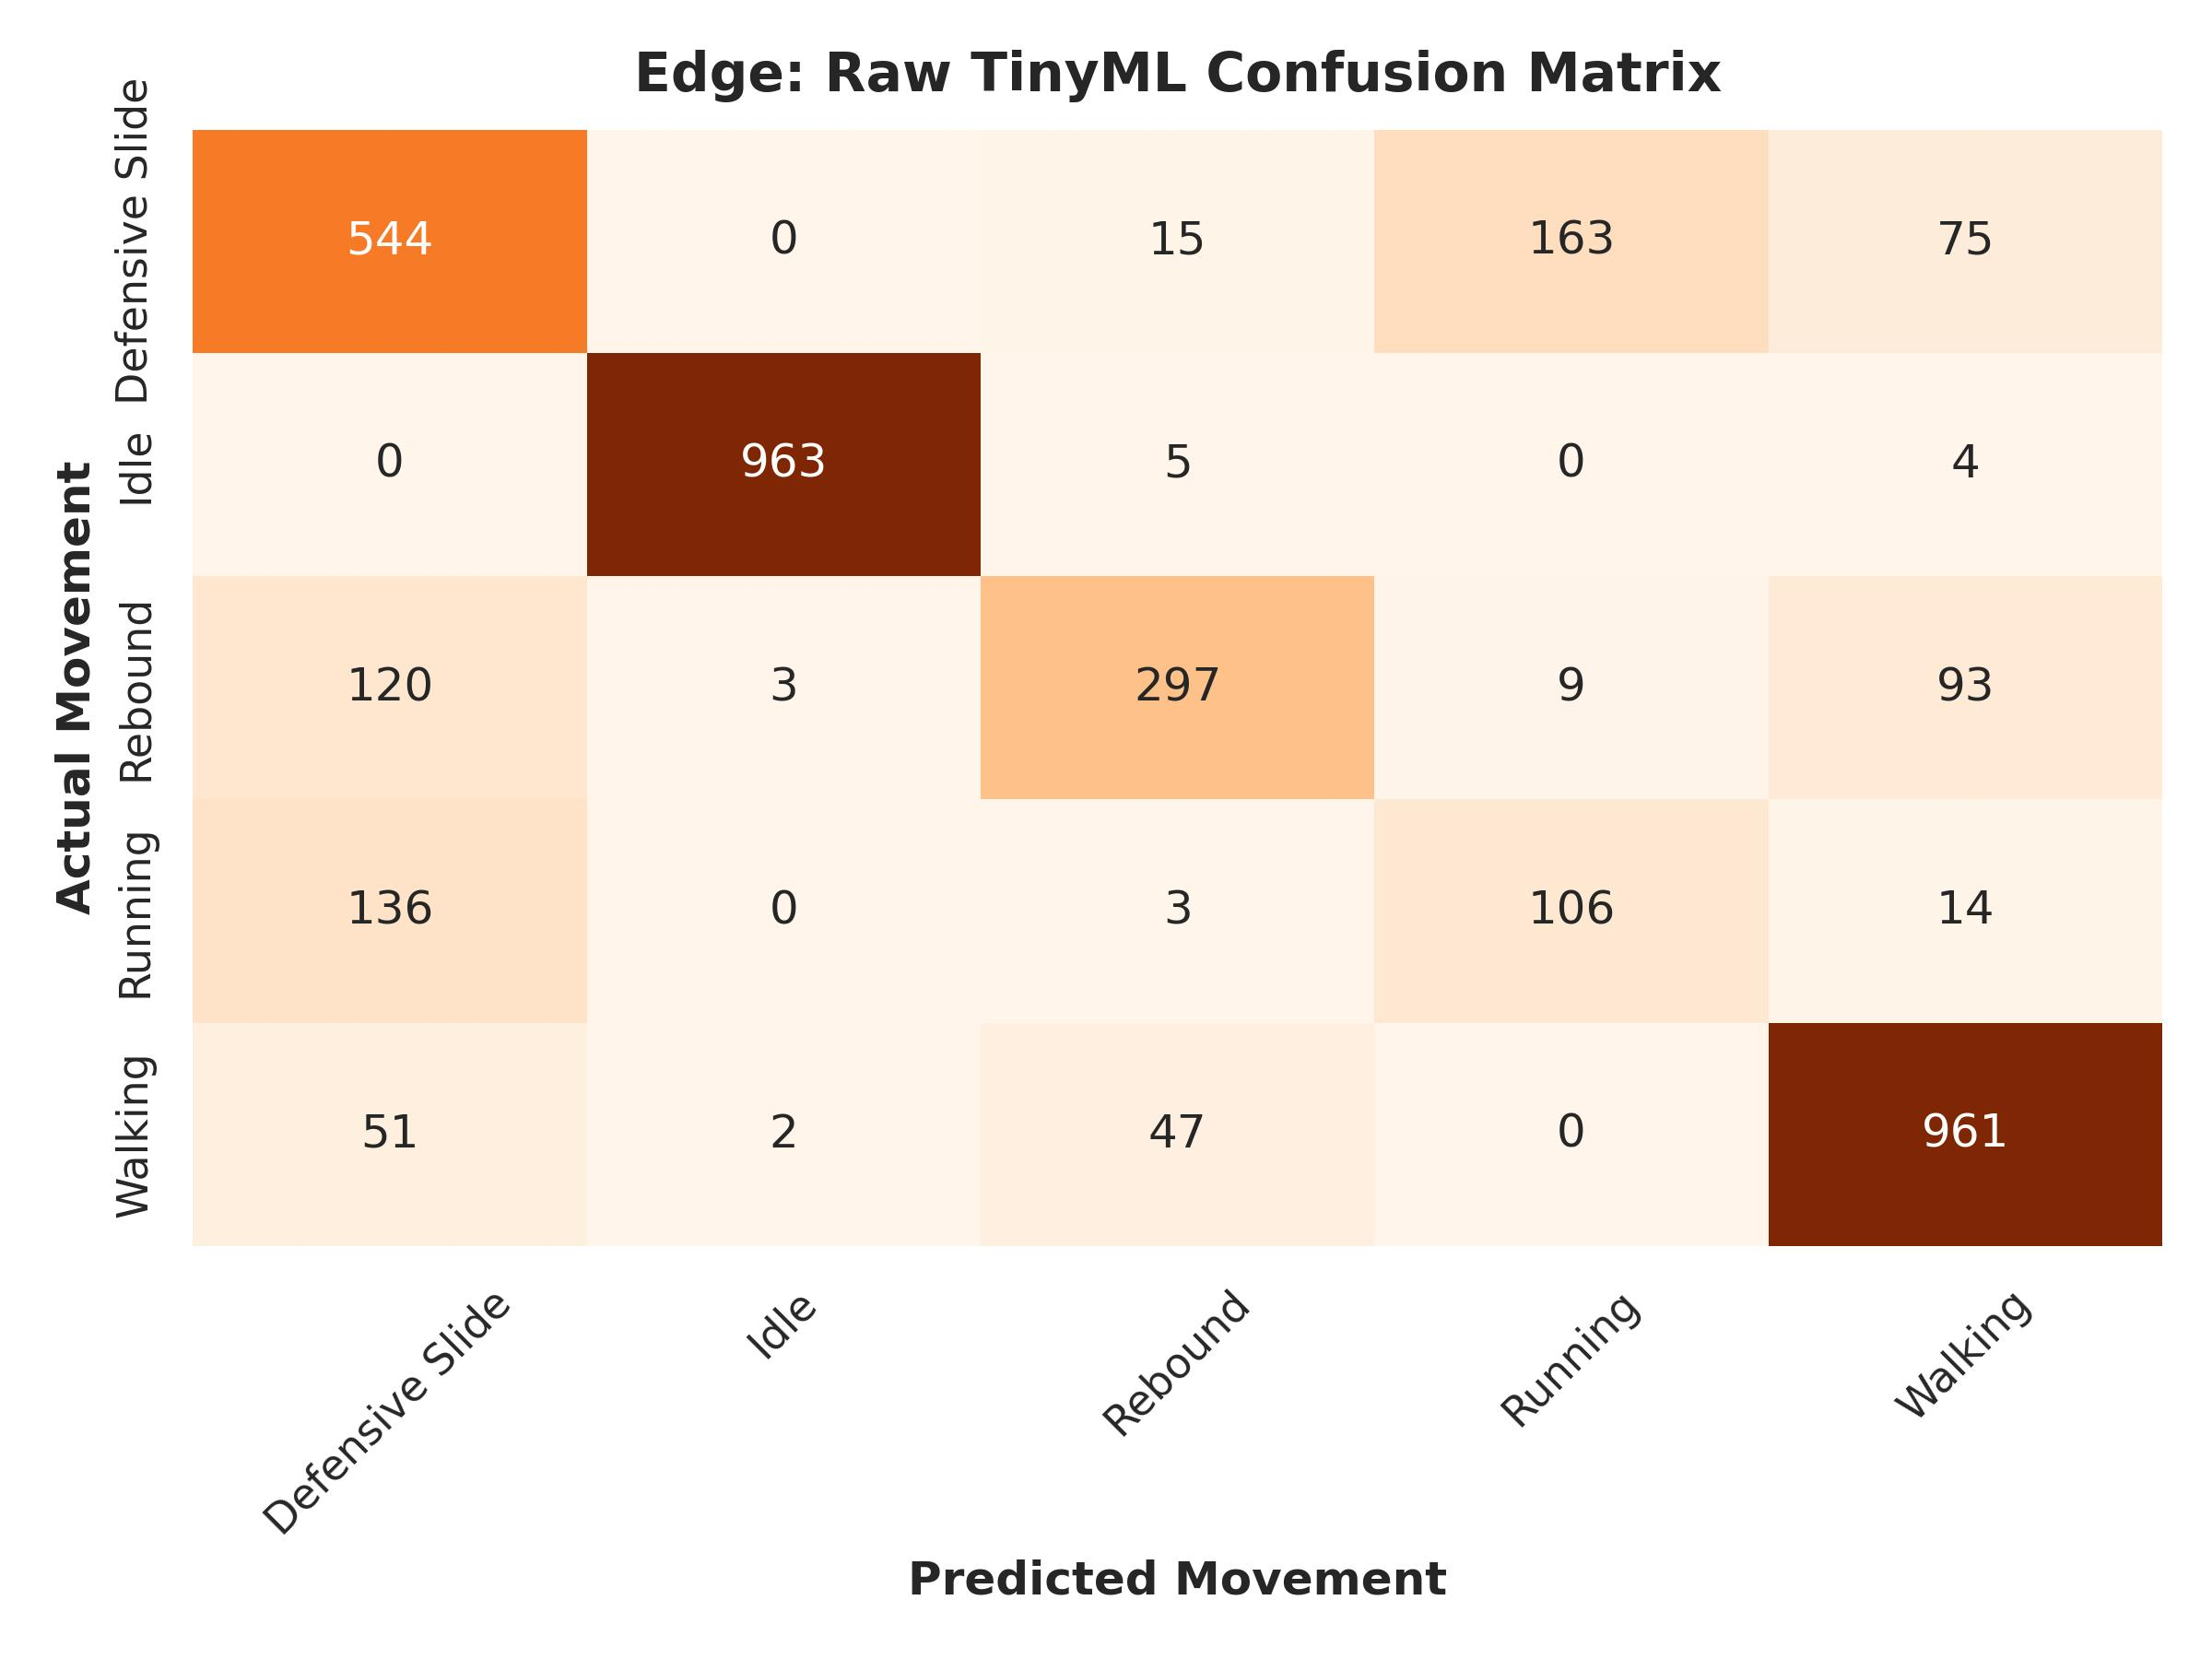
\includegraphics[width=\linewidth]{testConfusionMatrixTinyMLRaw.jpg}}
\caption{TinyML Confusion Matrix.}
\label{CFRaw}
\end{figure}

\begin{figure}[b]
\centerline{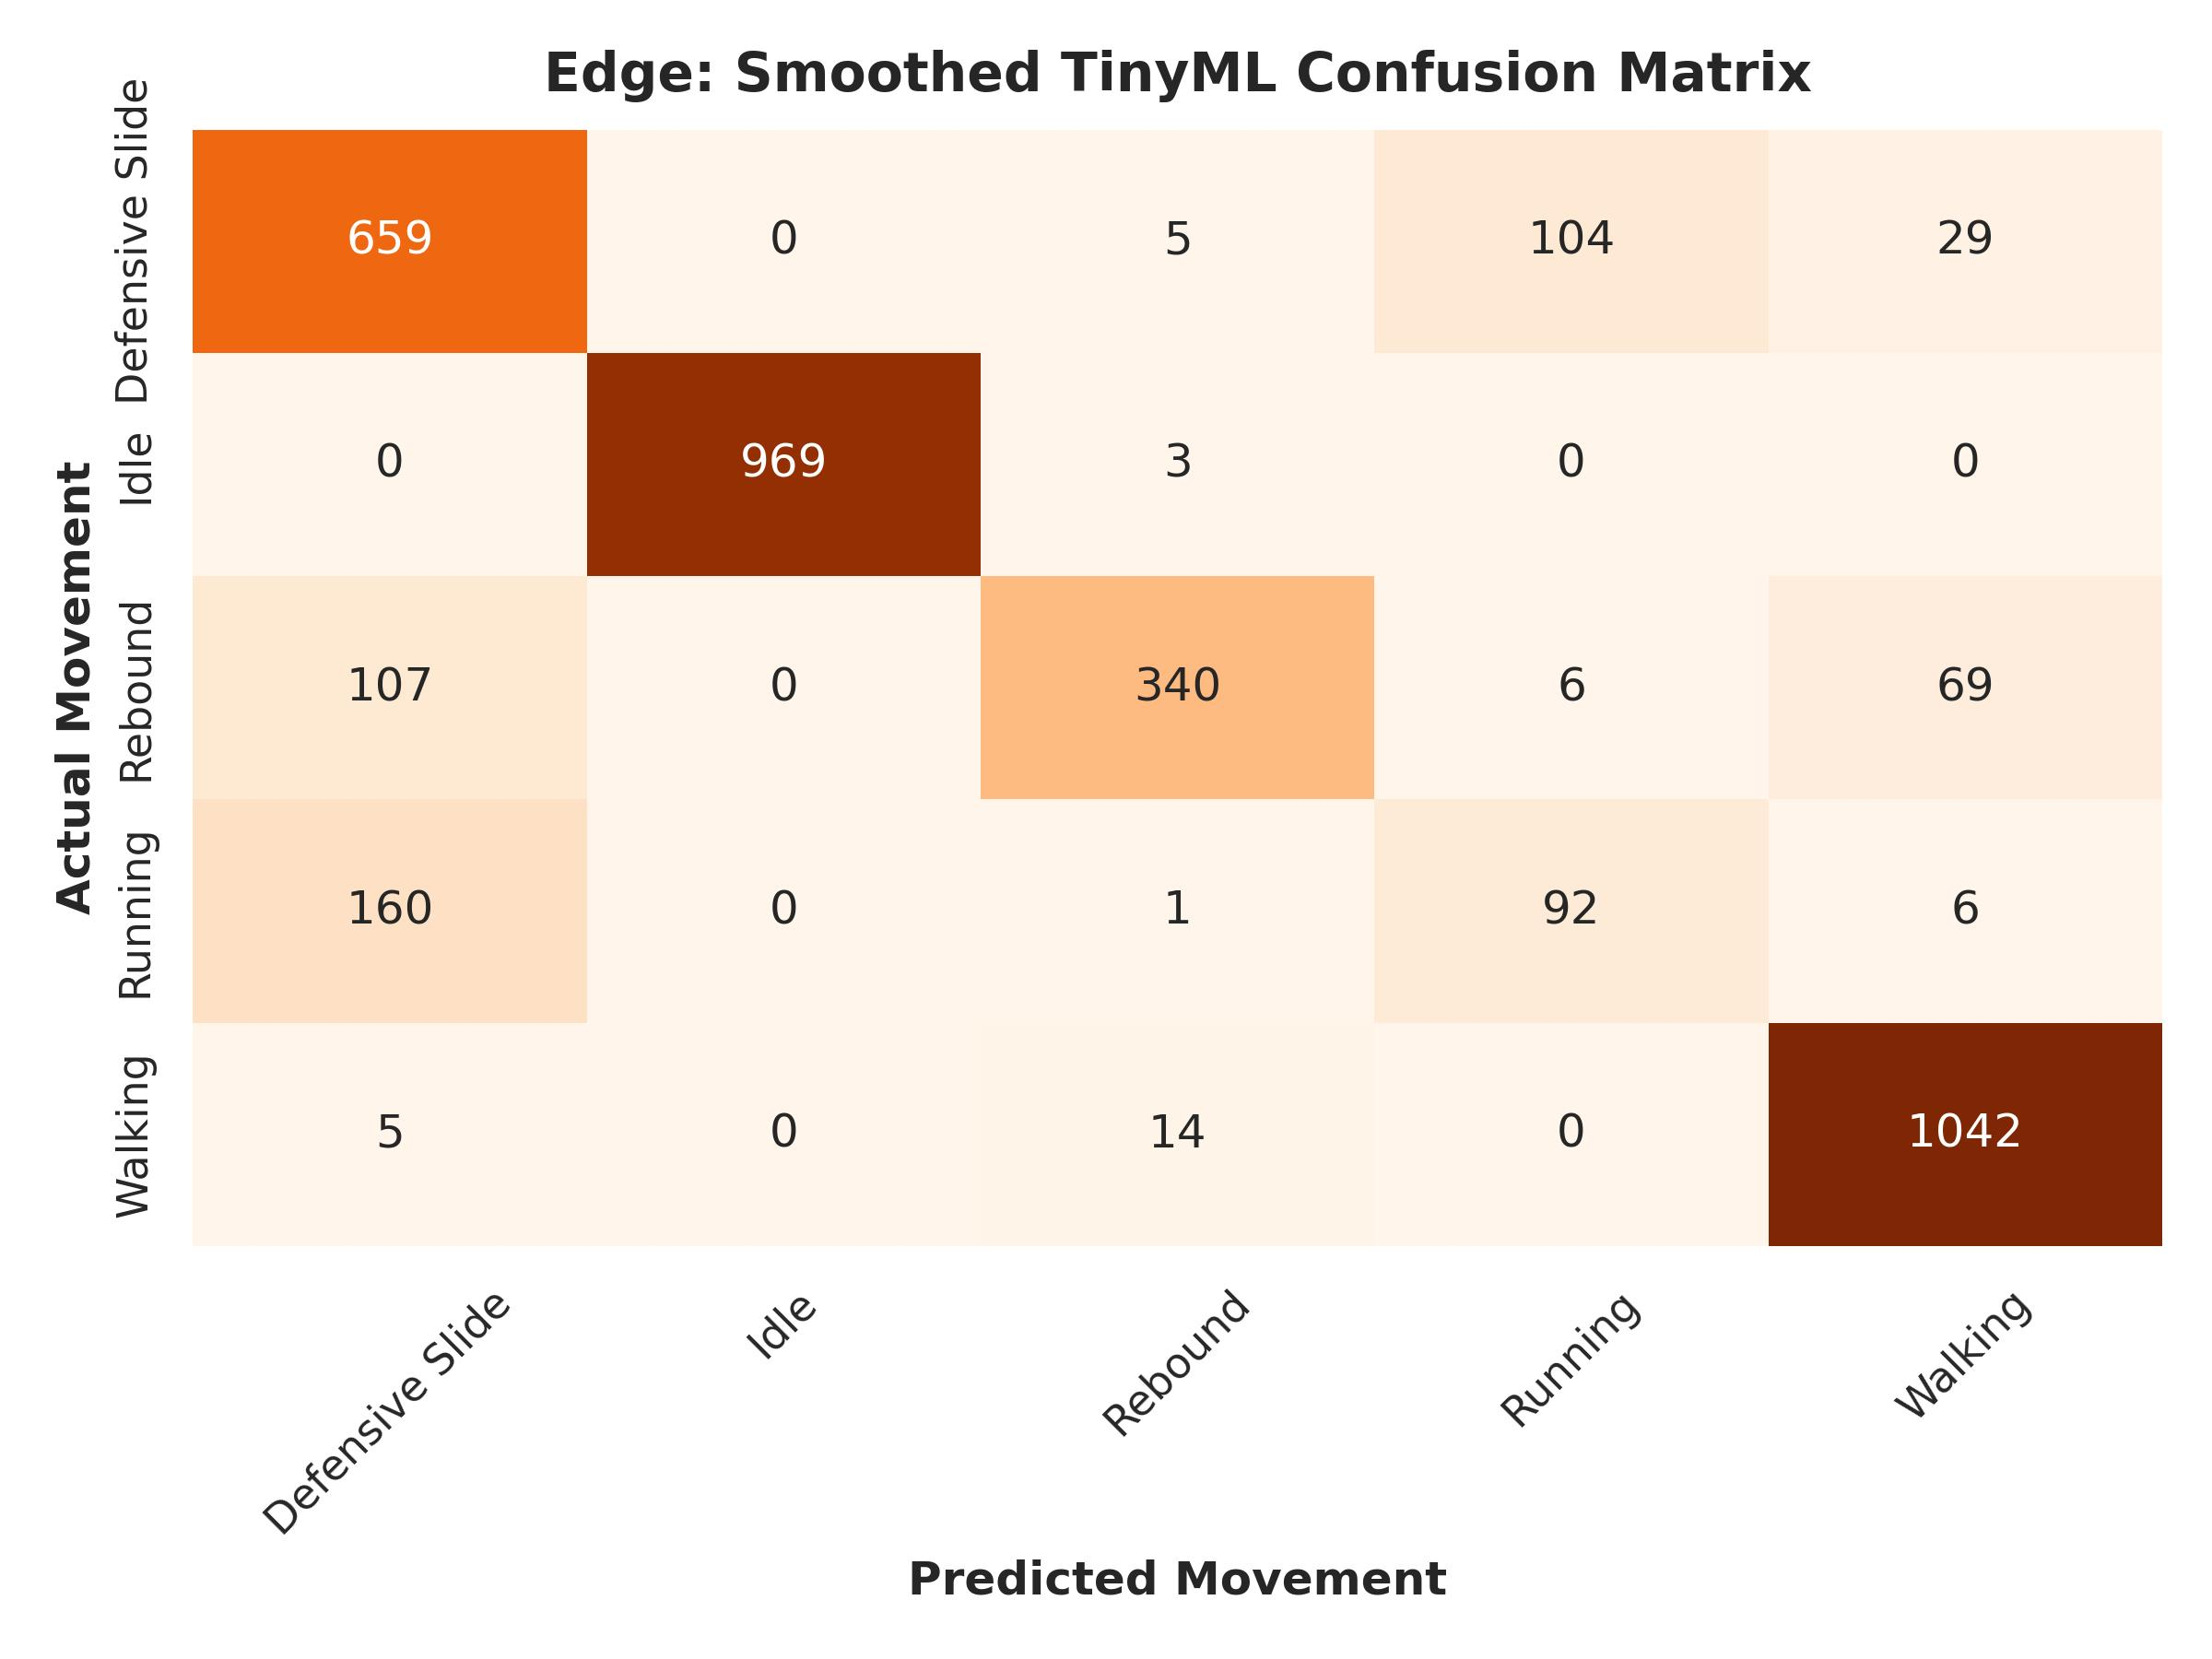
\includegraphics[width=\linewidth]{testConfusionMatrixTinyMLSmoothed.jpg}}
\caption{TinyML with Smoothing Confusion Matrix.}
\label{CFSmoothed}
\end{figure}

\section{Discussion and Know Limitations}

The experimental results validate the core hypothesis that integrating EMG with IMU data significantly enhances movement recognition. Feature Importance analysis confirms that RF classifier prioritized the features
VAR and RMS over kinematic data to resolve biomechanical similarities between movements.

Furthermore, the 500ms Majority Voting window proved to be an effective digital low-pass filter, increasing "Idling" accuracy by 6.4\%. However, this introduces a localized "responsiveness-stability" trade-off. 
While the resulting latency is acceptable for general activity tracking and fatigue monitoring, the suppression of explosive movements (e.g., rebounds) suggests that future iterations should employ adaptive 
windowing to maintain sensitivity.

The transition to live basketball testing exposed critical durability issues. The mechanical stress exerted by the wires ripped the USB port of one prototype, necessitating manual hardware reinforcement. Furthermore, 
the prototype occasionally shifted, introducing mechanical noise. Data integrity for the left limb was specifically impacted by a degradation in the BLE antenna range following hardware strain, leading to periodic 
packet loss when the android device was not in immediate proximity. Ergonomically, the external power management circuit caused minor discomfort, 
indicating that a transition to fully integrated, soft-shell enclosures is necessary for long-term athletic use.

The current dataset faces generalizability constraints due to the limited sample size. The models are likely tuned to the specific biomechanical signatures of the test subjects, requiring a broader demographic pool 
for universal validation. Additionally, the manual labeling process introduced "boundary noise" during movement transitions, slightly affecting training data purity. Finally, the physiological capture of pre-cramp 
states proved difficult to reproduce safely and consistently. This resulted in challenges for establishing a sustained RMS baseline, making the fatigue monitoring alerts highly sensitive to individual calibration.

\section{Conclusion}

In summary, the localized TinyML model outperformed the Cloud-tier RF (79.5\% vs 71.2\% accuracy), while providing the instantaneous feedback required for injury prevention. The implementation of a 500ms 
majority-voting algorithm successfully improved classifications despite the identified trade-off in sensitivity regarding explosive movements like rebounds.

Future work will focus on transitioning the prototype into a fully integrated smart-textile garment to improve ergonomics and signal stability. Additionally, expanding the dataset demographic and correlating EMG 
threshold breaches with clinical physiological markers will further refine the system's predictive accuracy and universal applicability.


%\begin{equation}
%a+b=\gamma\label{eq}
%\end{equation}



%\paragraph{Positioning Figures and Tables} Place figures and tables at the top and 
%bottom of columns. Avoid placing them in the middle of columns. Large 
%figures and tables may span across both columns. Figure captions should be 
%below the figures; table heads should appear above the tables. Insert 
%figures and tables after they are cited in the text. Use the abbreviation 
%``Fig.~\ref{fig}'', even at the beginning of a sentence.


%\section*{Acknowledgment}

%The preferred spelling of the word ``acknowledgment'' in America is without 
%an ``e'' after the ``g''. Avoid the stilted expression ``one of us (R. B. 
%G.) thanks $\ldots$''. Instead, try ``R. B. G. thanks$\ldots$''. Put sponsor 
%acknowledgments in the unnumbered footnote on the first page.



%Please number citations consecutively within brackets \cite{b1}. The 
%sentence punctuation follows the bracket \cite{b2}. Refer simply to the reference 
%number, as in \cite{b3}---do not use ``Ref. \cite{b3}'' or ``reference \cite{b3}'' except at 
%the beginning of a sentence: ``Reference \cite{b3} was the first $\ldots$''

%Number footnotes separately in superscripts. Place the actual footnote at 
%the bottom of the column in which it was cited. Do not put footnotes in the 
%abstract or reference list. Use letters for table footnotes.

%Unless there are six authors or more give all authors' names; do not use 
%``et al.''. Papers that have not been published, even if they have been 
%submitted for publication, should be cited as ``unpublished'' \cite{b4}. Papers 
%that have been accepted for publication should be cited as ``in press'' \cite{b5}. 
%Capitalize only the first word in a paper title, except for proper nouns and 
%element symbols.


\begin{thebibliography}{00}
\bibitem{b1} Lutz, Jonas \& Memmert, Daniel \& Raabe, Dominik \& Dornberger, Rolf \& Donath, Lars. (2019). Wearables for Integrative Performance and Tactic Analyses: Opportunities, Challenges, and Future Directions. International Journal of Environmental Research and Public Health. 17. 59. 10.3390/ijerph17010059. 
\bibitem{b6} Hwang, Soree \& Kwon, Nayeon \& Lee, Dongwon \& Kim, Jongman \& Yang, Sumin \& Youn, Inchan \& Moon, Hyuk-June \& Sung, Joon-Kyung \& Han, Sungmin. (2025). A Multimodal Fatigue Detection System Using sEMG and IMU Signals with a Hybrid CNN-LSTM-Attention Model. Sensors. 25. 3309. 10.3390/s25113309. 
\bibitem{b9} Otálora S, Segatto MEV, Monteiro ME, Múnera M, Díaz CAR, Cifuentes CA. Data-Driven Approach for Upper Limb Fatigue Estimation Based on Wearable Sensors. Sensors (Basel). 2023 Nov 20;23(22):9291. doi: 10.3390/s23229291.
\bibitem{b5} Baigarayeva, Zhanel \& Boltaboyeva, Assiya \& Imanbek, Baglan \& Ozhikenov, Kassymbek \& Karymssakova, Nurgul \& Beisembekova, Roza. (2025). Machine learning-based classification of local muscle fatigue using electromyography signals for enhanced rehabilitation outcomes. International Journal of Electrical and Computer Engineering (IJECE). 15. 5954. 10.11591/ijece.v15i6.pp5954-5967. 
\bibitem{b2} Qassim, H.M.; Hasan, W.Z.W.; Ramli, H.R.; Harith, H.H.; Mat, L.N.I.; Ismail, L.I. Proposed Fatigue Index for the Objective Detection of Muscle Fatigue Using Surface Electromyography and a Double-Step Binary Classifier. Sensors 2022, 22, 1900. https://doi.org/10.3390/s22051900 
\bibitem{b4} Kamaruddin, Asyikin \& Khalid, Puspa Inayat \& Sha'ameri, A.Z.. (2015). The Use of Surface Electromyography in Muscle Fatigue Assessments-A Review. Jurnal Teknologi.  
\bibitem{b7} Seniam (Surface ElectroMyoGraphy for the Non-Invasive Assessment of Muscles) Project Website. url: http://seniam.org/
%\bibitem{b11} K. Eves and J. Valasek, ``Adaptive control for singularly perturbed systems examples,'' Code Ocean, Aug. 2023. [Online]. Available: https://codeocean.com/capsule/4989235/tree
\end{thebibliography}

%\vspace{12pt}
%\color{red}
%IEEE conference templates contain guidance text for composing and formatting conference papers. Please ensure that all template text is removed from your conference paper prior to submission to the conference. Failure to remove the template text from your paper may result in your paper not being published.

\end{document}
 